\chapter{Выполнение лабораторной работы}

\section{Индивидуальное задание}

\textbf{Вариант 19}

Входные данные содержатся в файле с названием
simulated\_blockmodel\newline\_graph\_500\_nodes.tsv. В каждой строке записаны два
номера вершин и вес ребра.




\section{Код программы}

\captionsetup{singlelinecheck = false, justification=raggedright}
\begin{lstlisting}[label=full2, caption=Изменённый фрагмент кода host\_main.cpp]
__foreach_core(group, core)
{
	lnh_inst.gpc[group][core]->start_async(__event__(delete_graph));
}


unsigned int* host2gpc_ext_buffer[LNH_GROUPS_COUNT][LNH_MAX_CORES_IN_GROUP];
unsigned int messages_count = 0;
unsigned int u, v, w;

__foreach_core(group, core)
{
	host2gpc_ext_buffer[group][core] = (unsigned int*)lnh_inst.gpc[group][core]->external_memory_create_buffer(16 * 1048576 * sizeof(int)); //2*3*sizeof(int)*edge_count);
	offs = 0;
	
	std::ifstream file(argv[3], std::ios::in);
	
	if (!file.is_open())
	{
		std::cout << "Cannot open input file." << std::endl;
		
		return EXIT_FAILURE;
	}
	
	for (std::string line; std::getline(file, line); ) 
	{
		std::vector<std::string> tokens = split(line, '\t');
		
		if (tokens.size() != 3)
		{
			std::cout << "Incorrect tokens count in file: expected 3, got " << tokens.size() << "." << std::endl;
			
			return EXIT_FAILURE;
		}
		
		u = std::stoul(tokens[0]);
		v = std::stoul(tokens[1]);
		w = std::stoul(tokens[2]);
		
		EDGE(u, v, w);
		EDGE(v, u, w);
		messages_count += 2;
	}
	
	lnh_inst.gpc[group][core]->external_memory_sync_to_device(0, 3 * sizeof(unsigned int)*messages_count);
}
__foreach_core(group, core)
{
	lnh_inst.gpc[group][core]->start_async(__event__(insert_edges));
}
__foreach_core(group, core) {
	long long tmp = lnh_inst.gpc[group][core]->external_memory_address();
	lnh_inst.gpc[group][core]->mq_send((unsigned int)tmp);
}
__foreach_core(group, core) {
	lnh_inst.gpc[group][core]->mq_send(3 * sizeof(int)*messages_count);
}


__foreach_core(group, core)
{
	lnh_inst.gpc[group][core]->finish();
}
printf("Data graph created!\n");
\end{lstlisting}


\section{Тестирование программного обеспечения}

\begin{figure}[h!]
	\begin{center}
		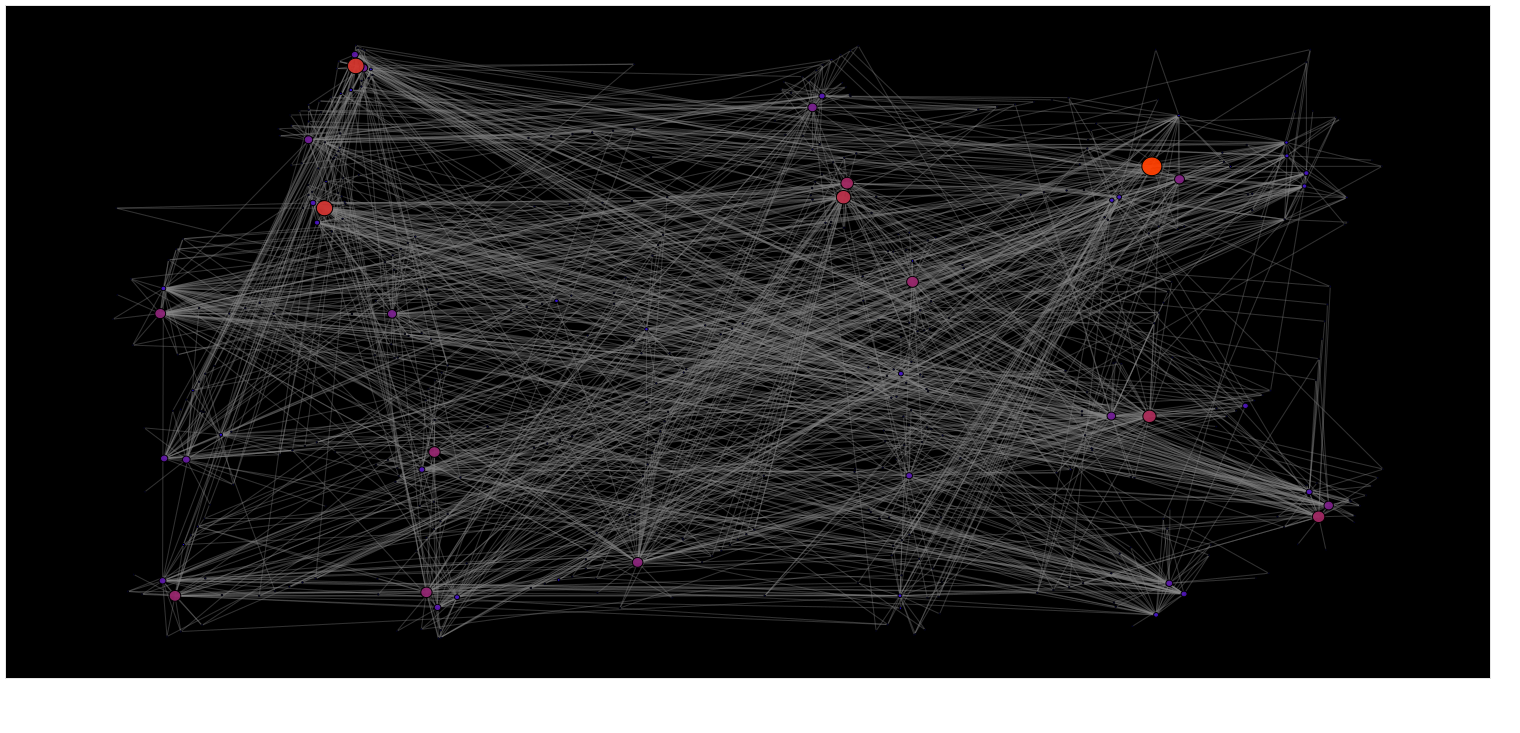
\includegraphics[width=0.95\textwidth]{img/1.png}
	\end{center}
	\caption{Раскладка сообществ с помощью иерархического объединения и укладки в боксы}
	\label{img:graph1}
\end{figure}

\begin{figure}[h!]
	\begin{center}
		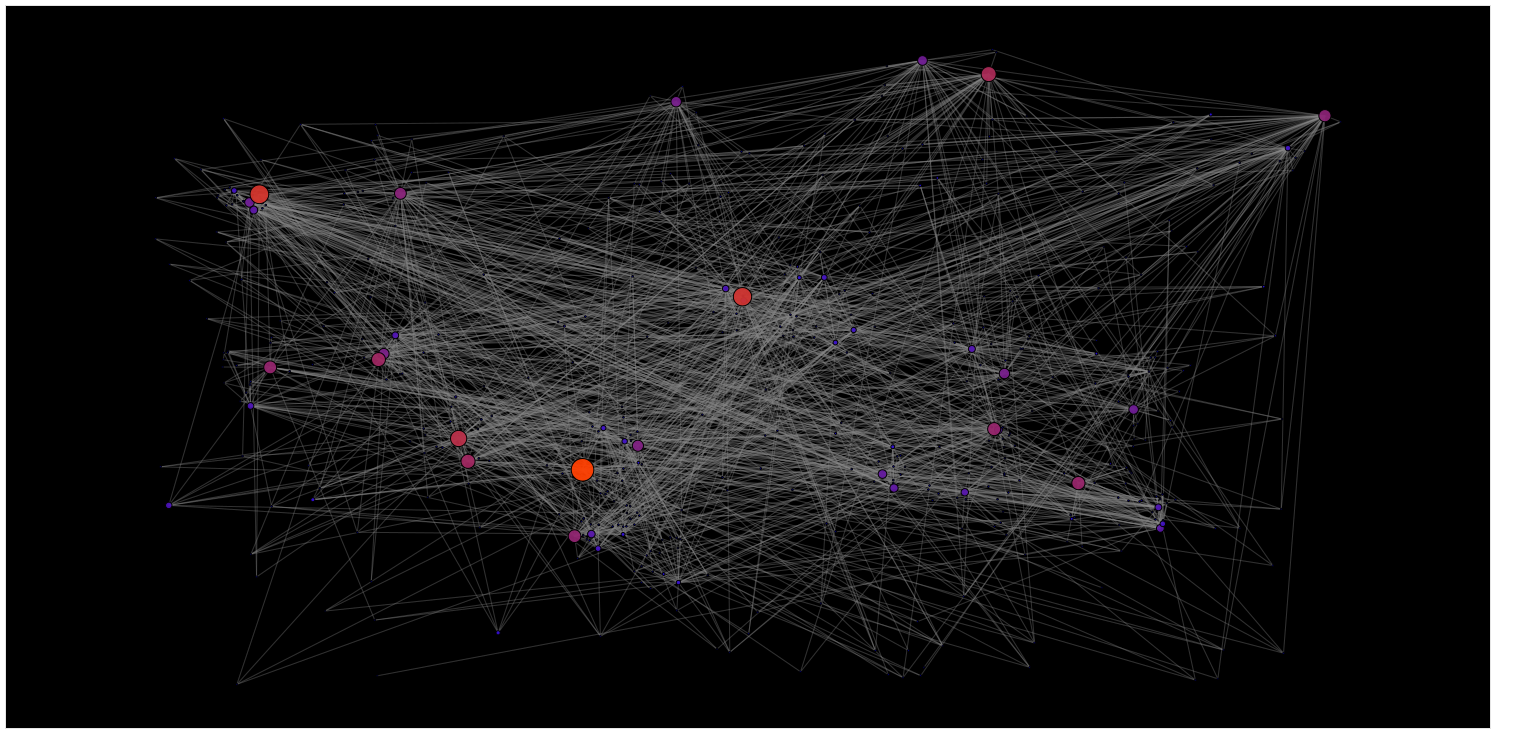
\includegraphics[width=0.95\textwidth]{img/2.png}
	\end{center}
	\caption{Раскладка сообществ с помощью силового алгоритма Фрухтермана-Рейнгольда}
	\label{img:graph2}
\end{figure}
